%{
% \documentclass[12pt, ngerman]{/Users/dominik-cau/Documents/Lernen/Uni/Promotion/Lehre/Latex-Vorlage/ExamClass}
% \documentclass[12pt, english]{AssignmentClass}
\documentclass[12pt, ngerman]{AssignmentClass}

%----------------------------------------------------------------------------------------
%	PACKAGES AND OTHER DOCUMENT CONFIGURATIONS
%----------------------------------------------------------------------------------------

% Template-specific packages
\usepackage[utf8]{inputenc} % Required for inputting international characters
\usepackage[T1]{fontenc} % Output font encoding for international characters
\usepackage{mathpazo} % Use the Palatino font
\usepackage{graphicx} % Required for including images
\usepackage{amsmath}
\usepackage{booktabs} % Required for better horizontal rules in tables
\usepackage[normalem]{ulem}
\usepackage{listings} % Required for insertion of code
\usepackage{siunitx}
\usepackage{array}
\usepackage{pnets}
\newcolumntype{Y}{>{\centering\arraybackslash}X}
\newcolumntype{C}[1]{>{\centering\arraybackslash}p{#1}}
\usepackage{comment}
\DeclareMathAlphabet{\mathpzc}{OT1}{pzc}{m}{it}
\useunder{\uline}{\ul}{}

\usepackage[utf8]{inputenc}

% Default fixed font does not support bold face
\DeclareFixedFont{\ttb}{T1}{txtt}{bx}{n}{12} % for bold
\DeclareFixedFont{\ttm}{T1}{txtt}{m}{n}{12}  % for normal

% Custom colors
\usepackage{color}
\definecolor{deepblue}{rgb}{0,0,0.5}
\definecolor{deepred}{rgb}{0.6,0,0}
\definecolor{deepgreen}{rgb}{0,0.5,0}

% Listings and python code
\usepackage{listings}
\usepackage{xcolor}
\definecolor{commentgreen}{rgb}{0,0.6,0}
\definecolor{keywordblue}{rgb}{0,0,0.8}
\definecolor{stringred}{rgb}{0.6,0,0}
\lstset{
    language=Python,
    basicstyle=\ttfamily\scriptsize, % Reduced font size
    keywordstyle=\color{keywordblue}\bfseries,
    stringstyle=\color{stringred},
    commentstyle=\color{commentgreen}\itshape,
    showstringspaces=false,
    numbers=left,
    numberstyle=\tiny,
    breaklines=true,
    frame=single,
    rulecolor=\color{black},
    xleftmargin=0pt, % No extra margin on the left
    framexleftmargin=0pt
}

% Underline %
\usepackage{contour}
\usepackage{ulem}

% new column types
\usepackage{array}
\newcolumntype{L}[1]{>{\raggedright\let\newline\\\arraybackslash\hspace{0pt}}m{#1}}
\newcolumntype{C}[1]{>{\centering\let\newline\\\arraybackslash\hspace{0pt}}m{#1}}
\newcolumntype{R}[1]{>{\raggedleft\let\newline\\\arraybackslash\hspace{0pt}}m{#1}}
\usepackage{graphicx,multirow}
\usepackage{wrapfig}
\setlength\intextsep{0pt}
\usepackage{stackengine}
\newcommand\xrowht[2][0]{\addstackgap[.5\dimexpr#2\relax]{\vphantom{#1}}}

% table
\usepackage{multirow}
\usepackage{tabularx}

% no indent
\setlength\parindent{0pt}

\renewcommand{\ULdepth}{1.8pt}
\contourlength{0.8pt}

\newcommand{\fancyuline}[1]{%
	\uline{\phantom{#1}}%
	\llap{\contour{white}{#1}}%
}

%----------------------------------------------------------------------------------------
%	ASSIGNMENT INFORMATION
%----------------------------------------------------------------------------------------
	
% \title{Hauptklausur} % Assignment title
\title{Matrikelnummer:} % Assignment title
\class{Generative KI} % Course or class name
\term{Sommersemester 2024 -- Nebenklausur} % Footer Line

% Exam Version
% \includecomment{answerbox}
% \excludecomment{solution}
% Solution Version
\excludecomment{answerbox}
\includecomment{solution}
%}

\begin{document}

\section*{Aufgabe 1 (Generative KI) \hfill 16 Punkte}

    % Aufgabenteil a
    \begin{enumerate}[a)]
		\item 
			\begin{minipage}[t]{\linewidth}
				\vspace{-0.61em}
				\begin{wrapfigure}[2]{r}{0.18\linewidth} 
					\raggedleft
					\texttt{(6 Punkte)}
				\end{wrapfigure}
                Geben Sie vier risikoreiche Einsatzfelder für Generative KI an. Beschreiben Sie zwei der vier risikoreichen Einsatzfelder. Wieso ist das ein Risikobereich?
			\end{minipage}
	\end{enumerate}
    
    \begin{answerbox}
		\noindent
		\fbox{\parbox[c]{\textwidth}{
				\vspace{3cm}
				\hspace{\textwidth}
		}}\\
	\end{answerbox}

	\begin{solution}
		\noindent
		\fbox{\parbox[c]{\textwidth}{
				\small
				\begin{tabular}{cp{13cm}}
					Punkte &\\
                    1,5 & Kriegstechnologie (0,5 P.): Einsatz von KI bei Schusswaffen. Im Falle von Schaden/Verletzungen ist nicht klar, wer hier verletzt hat. Hat die KI entschieden, dass Waffen eingesetzt werden? (1 P.)\\
                    1,5 & Forschung und Wissenschaft (0,5 P.): Einsatz von KI Trainingsdaten für nicht ethische Szenarien. Z.B. Genommutationen (1 P.)\\
                    1,5 & Überwachung und Ausgrenzung (0,5 P.): Einsatz von Kamerabildern für die Beeinträchtigung der Privatheit (1 P.)\\
                    1,5 & Jura/Gericht (0,5 P.): das KI-System diskriminiert oder trifft eine Fehlentscheidung weshalb jemand ins Gefängnis muss (1 P.)
				\end{tabular}
				\hspace{\textwidth}
		}}\\
	\end{solution}

    % Aufgabenteil b
    \begin{enumerate}[b)]
		\item 
			\begin{minipage}[t]{\linewidth}
				\vspace{-0.61em}
				\begin{wrapfigure}[2]{r}{0.18\linewidth} 
					\raggedleft
					\texttt{(4 Punkte)}
				\end{wrapfigure}
                Beschreiben Sie zwei Vorteile von Open Source LLMs, wenn sie bei der Programmierung von Software eingesetzt wird.
			\end{minipage}
	\end{enumerate}
 
    \begin{answerbox}
		\noindent
		\fbox{\parbox[c]{\textwidth}{
				\vspace{4cm}
				\hspace{\textwidth}
		}}\\
	\end{answerbox}

	\begin{solution}
		\noindent
		\fbox{\parbox[c]{\textwidth}{
				\small
				\begin{tabular}{cp{13cm}}
					Punkte &\\
                    & Pro Vorteil 1 Punkt + 1 Punkt für Erklärung\\
                    2 & Keine Lizenzgebühren: können von beliebigen Personen ohne Lizenzgebühren eingesetzt werden\\
                    2 & Transparenz und Anpassbarkeit: durch die öffentliche Zugänglichkeit ist Transparenz und Anpassbarkeit des Quellcodes sehr leicht möglich\\
                    2 & Keine Abhängigkeit von einem Hersteller\\
                    2 & Interoperabilität durch offene Standards und Dateiformate
				\end{tabular}
				\hspace{\textwidth}
		}}\\
	\end{solution}

    % Aufgabenteil c
    \begin{enumerate}[c)]
		\item 
			\begin{minipage}[t]{\linewidth}
				\vspace{-0.61em}
				\begin{wrapfigure}[2]{r}{0.18\linewidth} 
					\raggedleft
					\texttt{(6 Punkte)}
				\end{wrapfigure}
                Geben Sie jeweils drei Beispiele, wo KI einem Menschen überlegen ist und wo der Mensch der KI überlegen ist (d.h., er/sie besser kann).  Tragen Sie die Beispiele für Überlegenheit der KI in die linke Spalte ein und die Überlegenheit des Menschen gegenüber der KI in der rechten Spalte ein.                
			\end{minipage}
	\end{enumerate}

    % Task Table
    % \begin{table}[h]
    %     \begin{tabularx}{\textwidth}{|p{0.45\textwidth}|X|}
    %     \hline
    %     \textbf{Leistung von KI} & \textbf{Menschliche Fähigkeiten} \\ \hline
    %     \multirow{3}{*}{} & \\ 
    %                       & \\ 
    %                       & \\ 
    %                       & \\ 
    %                       & \\ \hline
    %     \multirow{3}{*}{} & \\ 
    %                       & \\ 
    %                       & \\ 
    %                       & \\ 
    %                       & \\ \hline
    %     \multirow{3}{*}{} & \\ 
    %                       & \\ 
    %                       & \\ 
    %                       & \\ 
    %                       & \\ \hline
    %     \end{tabularx}
    % \end{table}

    % Solution Table
	\begin{solution}
        \begin{table}[h]
            \begin{tabularx}{\textwidth}{|p{0.45\textwidth}|X|}
            \hline
            \textbf{Leistung von KI} & \textbf{Menschliche Fähigkeiten} \\ \hline
            \multirow{3}{*}{} & \\
                              kontinuierlich kann Output & ethische Implikationen erkennen\\ 
                              generiert werden & \\ 
                              & \\ 
                              & \\ \hline
            \multirow{3}{*}{} & \\ 
                              große (Text)Daten sehr effizient & überprüfen, ob etwas in der realen \\ 
                              verarbeiten und Muster erkennen & Welt wahr ist \\ 
                              & \\ 
                              & \\ \hline
            \multirow{3}{*}{} & \\ 
                              Texte sehr schnell zusammenfassen & empathisch handeln und eine \\ 
                              oder neue Bilder, Videos erstellen & individuelle, menschliche Perspektive \\ 
                              & einnehmen \\ 
                              & \\ \hline
            \end{tabularx}
        \end{table}
	\end{solution}

\newpage

\section*{Aufgabe 2 (LLMs \& Prompt Engineering) \hfill 11 Punkte}

    % Aufgabenteil a
    \begin{enumerate}[a)]
		\item 
			\begin{minipage}[t]{\linewidth}
				\vspace{-0.61em}
				\begin{wrapfigure}[2]{r}{0.18\linewidth} 
					\raggedleft
					\texttt{(5 Punkte)}
				\end{wrapfigure}
                Ein neues Large Language Model soll initial mittels Supervised Learning trainiert werden.\\
                1) Woher werden die benötigten Daten bezogen?\\
                2) Wie werden aus gegebenen Texten die Satzstrukturen und Wahrscheinlichkeiten von Wortfolgen gewonnen?\\
                3) Erklären Sie zwei Probleme, die bei der Datenauswahl entstehen können, und wie man Ihnen begegnen sollte.
			\end{minipage}
	\end{enumerate}
 
	\begin{solution}
		\noindent
		\fbox{\parbox[c]{\textwidth}{
				\small
				\begin{tabular}{cp{13cm}}
					Punkte &\\
                    1 & Zu 1): Es werden große Datenmengen aus dem öffentlich zugänglichen Internet (Sammlungen von Webpages, Zeitungen, Bücher etc) bezogen. (F3, S.7)\\
                    2 & Zu 2): Texte werden Satz für Satz betrachtet. Teile des Satzes werden abgeschnitten/verdeckt/maskiert. Der verbleibende Satzteil und der verdeckte Satzteil bilden ein Frage-Antwort-Paar, das dem LLM präsentiert wird. Durch verschieben des verdeckten Teils kann ein einzelner Satz mehrere Frage-Antwort-Paare bilden. (F3, S.6)\\
                    1 & Zu 3): (Bsp.) Datenbias - es werden ungleich verteile Daten gelernt, was dazu führt, dass ein LLM bestimmte Antworten bevorzugt und andere diskriminiert. Eine ausgewogene Datengrundlage ist notwendig. (F1, S.18)\\
                    1 & Zu 3): (Bsp.) Zeitpunkt des Datendestands - ein LLM kann nicht erkennen, ob Jens Spahn immernoch Bundesgesundheitsminister ist. Ein LLM müsste Daten auch wieder "verlernen" können. (F1, S.18)
				\end{tabular}
				\hspace{\textwidth}
		}}\\
	\end{solution}

    \begin{answerbox}
		\noindent
		\fbox{\parbox[c]{\textwidth}{
				\vspace{6cm}
				\hspace{\textwidth}
		}}\\
	\end{answerbox}

    % Aufgabenteil b -- Prompt Engineering
    \begin{enumerate}[b)]
		\item 
			\begin{minipage}[t]{\linewidth}
				\vspace{-0.61em}
				\begin{wrapfigure}[2]{r}{0.18\linewidth} 
					\raggedleft
					\texttt{(6 Punkte)}
				\end{wrapfigure}
                Beschreiben Sie die vier Arten von Kontextinformationen, mit denen Sie den Inhalt einer Prompt-Antwort steuern können. Erstellen Sie zudem einen Zero-Shot Prompt, der alle Arten von Kontextinformationen berücksichtigt, um einen Projektpitch vor Kollegen und Vorgesetzten zu generieren.
			\end{minipage}
	\end{enumerate}

	\begin{solution}
		\noindent
		\fbox{\parbox[c]{\textwidth}{
				\small
				\begin{tabular}{cp{13cm}}
					Punkte & (alle: F3, S.34)\\
					1 & Zielgruppen, z.B. Geschäftspartner, Kunden, etc.\\
					1 & Format, z.B. Rede, PowerPoint, MindMap, etc.\\
                    1 & Tonalität, z.B. sachlich, wissenschaftlich, humorvoll, etc.\\
                    1 & Rolle (Sender), z.B. Mitarbeiter, Projektleiter, etc.\\
                    2 & (Ein nachvollziehbarer Prompt, der die o.g. Kontextinformationen verwendet)
				\end{tabular}
				\hspace{\textwidth}
		}}\\
	\end{solution}

    \begin{answerbox}
		\noindent
		\fbox{\parbox[c]{\textwidth}{
				\vspace{8cm}
				\hspace{\textwidth}
		}}\\
	\end{answerbox}


\section*{Aufgabe 3 (LLM-Anwendungen mit LangChain) \hfill 10 Punkte}
    In Ihrem Unternehmen ''erben'' Sie die Verantwortung für eine LLM-Anwendung, mit der in kurzer Zeit aus Produktideen Werbetexte erstellt werden. Weder wurde die Anwendung dokumentiert, noch ist der ursprüngliche Entwickler noch im Unternehmen.
    
    % \begin{figure}[h]
    %     \centering
    %     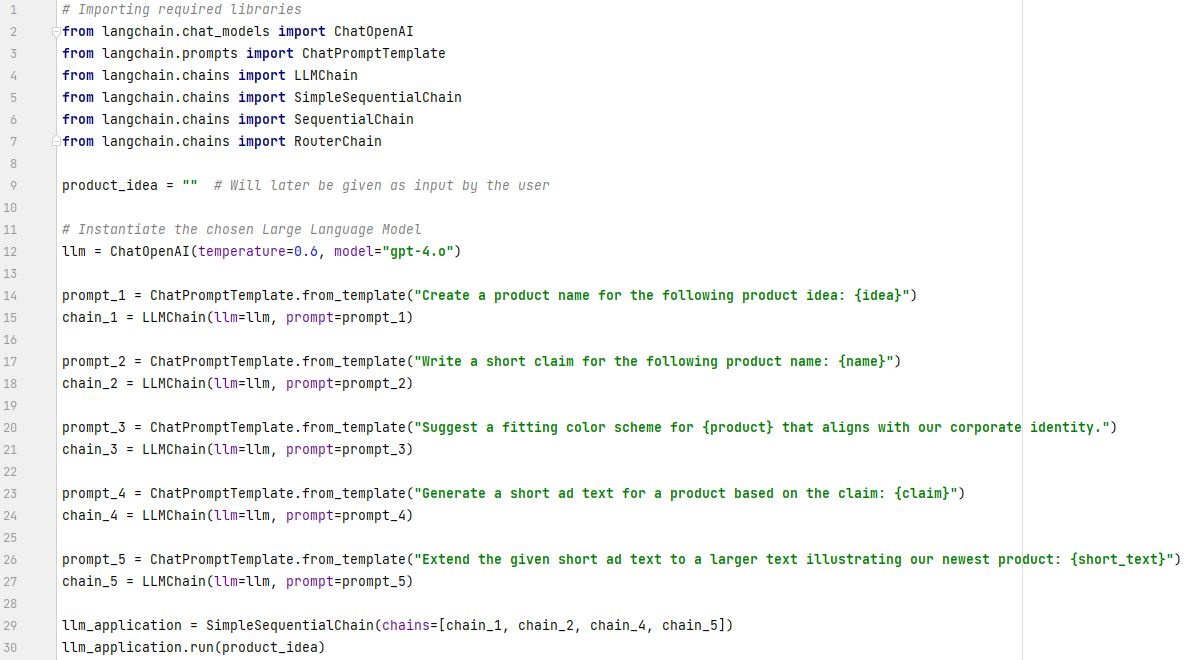
\includegraphics[width=0.9\linewidth]{media_nk/Aufgabe 3/Legacy Code White Mode.jpg}
    %     \caption{Aufgabe 3a): Code zur LLM-Anwendung}
    %     \label{fig:Aufgabe_3a}
    % \end{figure}

    \vspace{0.5cm}
    \begin{lstlisting}
        # Importing required libraries
        from langchain.chat_models import ChatOpenAI
        from langchain.prompts import ChatPromptTemplate
        from langchain.chains import LLMChain
        from langchain.chains import SimpleSequentialChain
        from langchain.chains import SequentialChain
        from langchain.chains import RouterChain
        
        product_idea = ""  # Will later be given as input by the user
        
        # Instantiate the chosen Large Language Model
        llm = ChatOpenAI(temperature=0.6, model="gpt-4.o")
        
        prompt_1 = ChatPromptTemplate.from_template(
            "Create a product name for the following product idea: {idea}")
        chain_1 = LLMChain(llm=llm, prompt=prompt_1)
        
        prompt_2 = ChatPromptTemplate.from_template(
            "Write a short claim for the following product name: {name}")
        chain_2 = LLMChain(llm=llm, prompt=prompt_2)
        
        prompt_3 = ChatPromptTemplate.from_template(
            "Suggest a fitting color scheme for {product} that aligns with our corporate identity.")
        chain_3 = LLMChain(llm=llm, prompt=prompt_3)
        
        prompt_4 = ChatPromptTemplate.from_template(
            "Generate a short ad text for a product based on the claim: {claim}")
        chain_4 = LLMChain(llm=llm, prompt=prompt_4)
        
        prompt_5 = ChatPromptTemplate.from_template(
            "Extend the given short ad text to a larger text illustrating our newest product: {short_text}")
        chain_5 = LLMChain(llm=llm, prompt=prompt_5)
        
        llm_application = SimpleSequentialChain(chains=[chain_1, chain_2, chain_4, chain_5])
        llm_application.run(product_idea)
    \end{lstlisting}

    % Aufgabenteil a -- Funktion von Code erkennen und beschreiben
    \begin{enumerate}[a)]
		\item 
			\begin{minipage}[t]{\linewidth}
				\vspace{-0.61em}
				\begin{wrapfigure}[2]{r}{0.18\linewidth} 
					\raggedleft
					\texttt{(2 Punkte)}
				\end{wrapfigure}
                Identifizieren Sie die von der LLM-Anwendung verwendeten LangChain-Komponenten und nennen Sie deren Funktionsweise.
			\end{minipage}
	\end{enumerate}

    \begin{answerbox}
		\noindent
		\fbox{\parbox[c]{\textwidth}{
				\vspace{6cm}
				\hspace{\textwidth}
		}}\\
	\end{answerbox}
    
	\begin{solution}
		\noindent
		\fbox{\parbox[c]{\textwidth}{
				\small
				\begin{tabular}{cp{13cm}}
					Punkte &\\
					1 & Eine SimpleSequentialChain (F4, S. 26, 27). Sie besteht wiederum aus mehreren Elementen und reicht den Output eines Elements als Input an das nachfolgende Element weiter bzw. gibt den letzten Output als Ergebnis aus.\\
                    1 & Vier LLMChains. Sie bestehen jeweils aus einem Promtp Template und einem LLM. Sie nehmen einen Input entgegen und liefern einen Output (F4, S.23, 24).\\
                    & \textbf{Hinweis:} Es werden zwar 5 LLMChain-Elemente instanziiert, die LLM-Anwendung verwendet aber nur 4 davon (chain\_3 wird gar nicht benutzt).
				\end{tabular}
				\hspace{\textwidth}
		}}\\
	\end{solution}

    % Aufgabenteil b -- LangChain modellieren
    \begin{enumerate}[b)]
		\item 
			\begin{minipage}[t]{\linewidth}
				\vspace{-0.61em}
				\begin{wrapfigure}[2]{r}{0.18\linewidth} 
					\raggedleft
					\texttt{(2 Punkte)}
				\end{wrapfigure}
                Erstellen Sie eine Skizze, um die Funktion der LLM-Anwendung zu visualisieren.
			\end{minipage}
	\end{enumerate}

    \begin{answerbox}
		\noindent
		\fbox{\parbox[c]{\textwidth}{
				\vspace{6cm}
				\hspace{\textwidth}
		}}\\
	\end{answerbox}

    \begin{figure}[h]
        \centering
        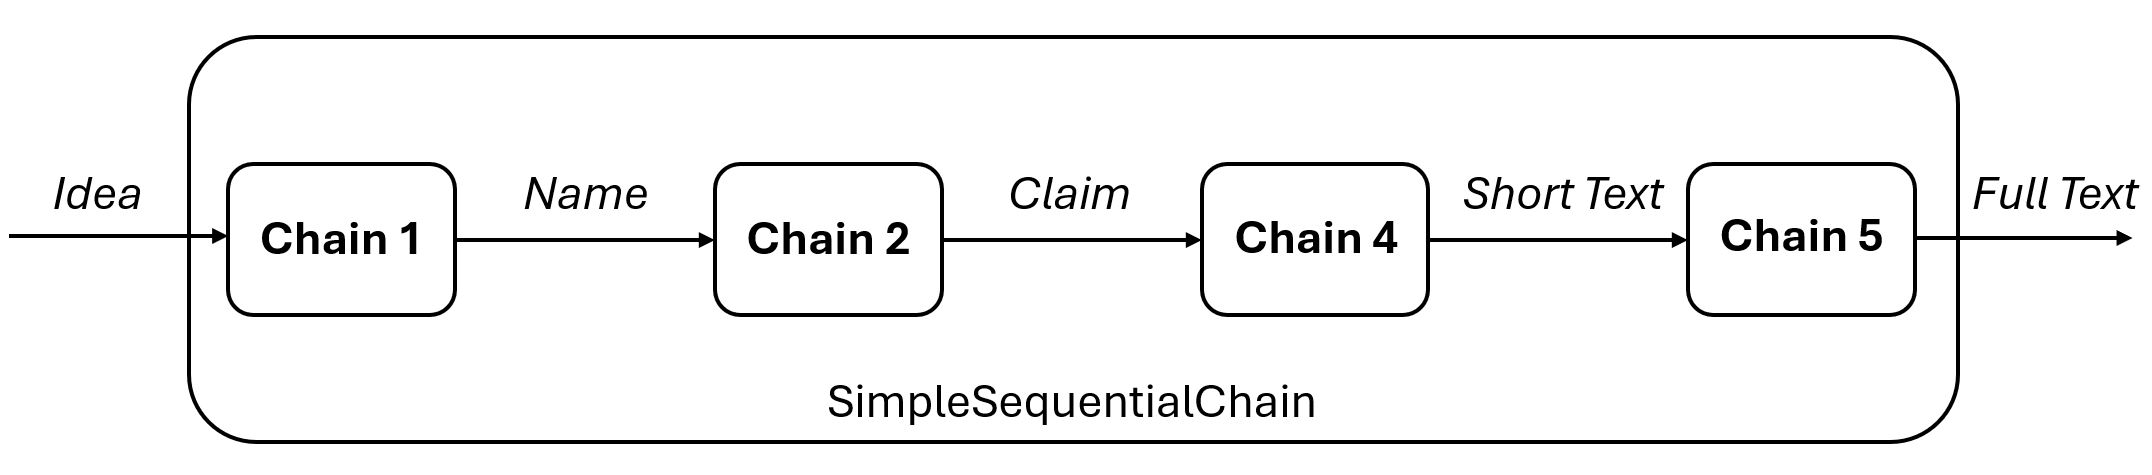
\includegraphics[width=1\linewidth]{media_nk/Aufgabe 3/Loesung-3b.jpg}
        \caption{Lösung zu Aufgabe 3b)}
        \label{fig:Loesung_3a}
    \end{figure}

    
    % Aufgabenteil c -- Architektonische Erweiterung des Codes
    \begin{enumerate}[c)]
		\item 
			\begin{minipage}[t]{\linewidth}
				\vspace{-0.61em}
				\begin{wrapfigure}[2]{r}{0.18\linewidth} 
					\raggedleft
					\texttt{(6 Punkte)}
				\end{wrapfigure}
                Ihr Vorgesetzter möchte die Möglichkeiten der Anwendung auch für andere Produktgruppen nutzen. Dazu soll in Abhängigkeit von der Produktidee wahlweise die bestehende Funktionalität genutzt, oder aber, wenn es um technische Produkte geht, folgendes generiert werden:\\
                Zur gegebenen Produktidee soll eine geeignete \textit{Farbpalette} für die Präsentation gewählt werden. Weiterhin soll ein geeigneter \textit{Claim} zur Produktidee generiert werden. Aus Farbpalette und Claim soll dann ein \textit{Werbebild} erstellt werden.\\
                Erstellen Sie eine grafische Skizze, die die neue Gesamtanwendung abbildet. Beschriften Sie Komponenten und Informationsflüsse. Sie brauchen keinen Code zu schreiben.
			\end{minipage}
	\end{enumerate}
 
	\begin{solution}
		\noindent
		\fbox{\parbox[c]{\textwidth}{
				\small
				\begin{tabular}{cp{13cm}}
					Punkte &\\
					1 & Die Architektur beginnt mit einem Router, der die Produktkategorie überprüft und die entsprechenden weiteren Chains aufruft (F4, S.31).\\
                    1 & Für die bisherige Funktionalität lässt sich die gesamte SSC aus Aufgabe 3a) wiederverwenden.\\
                    1 & Ein Router kann immer an der Aufgabenkategorisierung scheitern, daher benötigt man eine ''Default Chain'' für ''wenn das LLM nicht weiter weiß'' (F4, S. 31).\\
                    3 & Aufgabenteil 3c) ist korrekt in folgender Skizze umgesetzt:
				\end{tabular}
				\hspace{\textwidth}
		}}\\
	\end{solution}

    \begin{figure}[h]
        \centering
        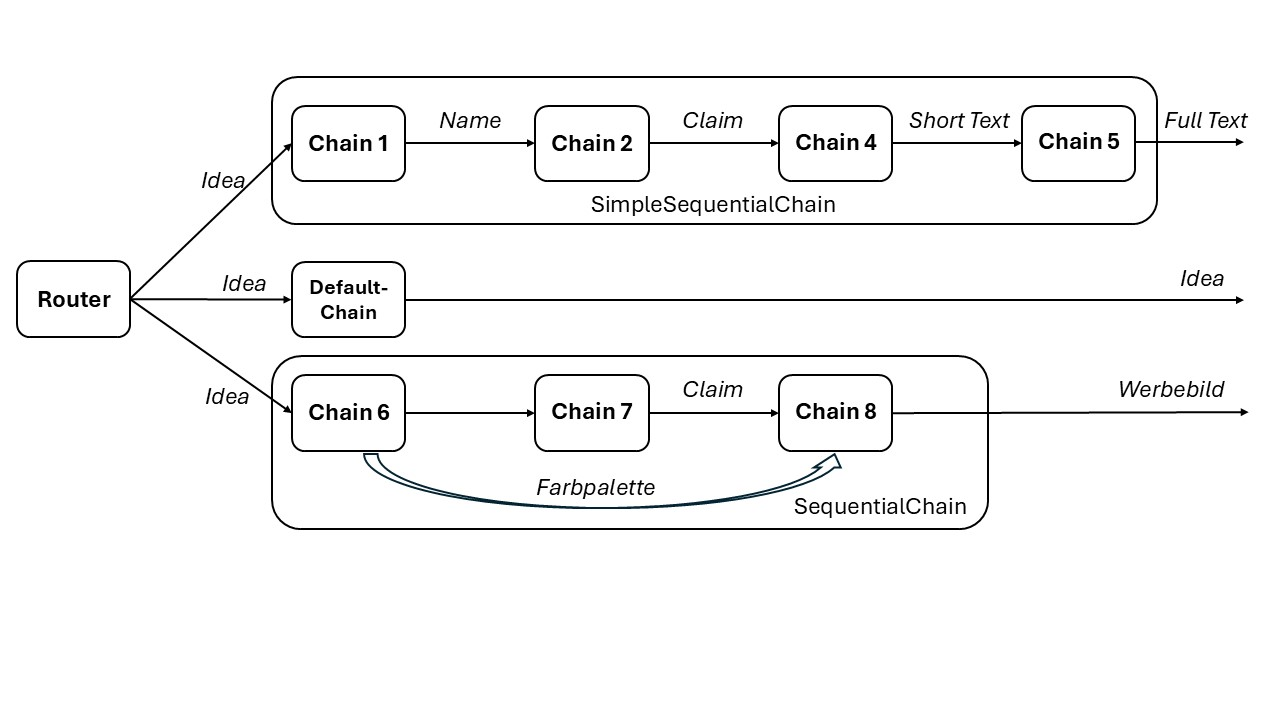
\includegraphics[width=1\linewidth]{media_nk/Aufgabe 3/Loesung_3c.JPG}
        \caption{Lösung zu Aufgabe 3c)}
        \label{fig:Loesung_3c}
    \end{figure}

    \begin{answerbox}
		\noindent
		\fbox{\parbox[c]{\textwidth}{
				\vspace{10cm}
				\hspace{\textwidth}
		}}\\
	\end{answerbox}

\newpage

\section*{Aufgabe 4 (Gastvorträge) \hfill 10 Punkte}

    % Aufgabenteil a
    \begin{enumerate}[a)]
		\item 
			\begin{minipage}[t]{\linewidth}
				\vspace{-0.61em}
				\begin{wrapfigure}[2]{r}{0.18\linewidth} 
					\raggedleft
					\texttt{(4 Punkte)}
				\end{wrapfigure}
                Im Gastvortrag von Herrn Prof. Peinl ("Multimodale KI - LLMs lernen sehen") ging es um die Evaluation von Bilderkennungsfähigkeiten Generativer KIs. Erlären Sie zwei Herausforderungen, die die Datenauswahl zum Training von Bilderkennung berücksichtigen muss.
			\end{minipage}
	\end{enumerate}

    \begin{solution}
		\noindent
		\fbox{\parbox[c]{\textwidth}{
				\small
				\begin{tabular}{cp{13cm}}
                    Punkte & \\
					2 & \textbf{Semantische Ähnlichkeit von Bildern:} Ähnliche Objekte (Rabe und Krähe, Delfin und Tümmler) sehen sehr ähnlich aus, sind aber unterschiedlich. Eine KI ist sich dieses Umstandes nicht bewusst und daher hier fehleranfällig.\\
					2 & \textbf{Datenverfügbarkeit aufgrund von regionaler/globaler Relevanz:} Für global relevante Personen und Objekte (z.B. Donald J. Trump) gibt es ausreichend Bildmaterial für eine hohe Erkennungsrate. Bei nur regional relevanten Personen und Objekten ist die Datengrundlage deutlich kleiner. Dies kann zu einer niedrigen Erkennungsrate führen.
				\end{tabular}
				\hspace{\textwidth}
		}}\\
	\end{solution}

    \begin{answerbox}
		\noindent
		\fbox{\parbox[c]{\textwidth}{
				\vspace{7cm}
				\hspace{\textwidth}
		}}\\
	\end{answerbox}

    % Aufgabenteil b
    \begin{enumerate}[b)]
		\item 
			\begin{minipage}[t]{\linewidth}
				\vspace{-0.61em}
				\begin{wrapfigure}[2]{r}{0.18\linewidth} 
					\raggedleft
					\texttt{(6 Punkte)}
				\end{wrapfigure}
                Die Entwicklung von Generativer KI stellt Forschung und Lehre vor neue Herausforderungen und bietet zugleich Potentiale. Beschreiben Sie drei potentielle Anwendungsgebiete, die in den Gastvorträgen adressiert wurden.
			\end{minipage}
	\end{enumerate}

    \begin{solution}
		\noindent
		\fbox{\parbox[c]{\textwidth}{
				\small
				\begin{tabular}{cp{13cm}}
                    Punkte & \\
                    2 & (Bsp.) Frage nach der Autorenschaft: Hat ein Autor (Wissenschaftler, Studierender) seine Arbeit überhaupt noch selbst verfasst? Wie kann das belastbar überprüft werden?\\
                    2 & (Bsp.) Glaubwürdigkeit von Ergebnissen: Wenn ich mir Sachverhalte und Zusammenhänge von einem LLM erklären lässt, kann ich dem Glauben? Wurden mir Halluzinationen untergejubelt?\\
                    2 & (Bsp.) Reproduzierbarkeit der Ergebnisse: Generative KI ist eine Blackbox, die in jedem Durchgang andere Ergebnisse/Formulierungen produziert. Basis von Wissenschaft ist die Überprüfbarkeit und Reproduzierbarkeit von Ergebnissen. Hier besteht ein grundlegender Konflikt.
				\end{tabular}
				\hspace{\textwidth}
		}}\\
	\end{solution}

    \begin{answerbox}
		\noindent
		\fbox{\parbox[c]{\textwidth}{
				\vspace{8cm}
				\hspace{\textwidth}
		}}\\
	\end{answerbox}

\newpage

\section*{Aufgabe 5 (Ethische, rechtliche und soziale Implikationen) \hfill 3 Punkte}
    Diskutieren Sie die ethischen, rechtlichen und sozialen Implikationen der Nutzung Generativer KI im Kontext der Arbeitswelt. Beziehen Sie sich in Ihrer Antwort auf folgende Aspekte:

    % Aufgabenteil a
    \begin{enumerate}[a)]
		\item 
			\begin{minipage}[t]{\linewidth}
				\vspace{-0.61em}
				\begin{wrapfigure}[2]{r}{0.18\linewidth} 
					\raggedleft
					\texttt{(1 Punkt)}
				\end{wrapfigure}
                Rechtliche Aspekte:\\
                Am 01.08.2024 trat der EU AI Act in Kraft. Wie werden darin KI-Systeme klassifiziert?
			\end{minipage}
	\end{enumerate}
 
	\begin{solution}
		\noindent
		\fbox{\parbox[c]{\textwidth}{
				\small
				\begin{tabular}{cp{13cm}}
					Punkte &\\
					1 & Es wird ein risikobasierter Ansatz verfolgt, der KI-Systeme in vier Risikoklassen eingruppiert.\\
				\end{tabular}
				\hspace{\textwidth}
		}}\\
	\end{solution}

    \begin{answerbox}
		\noindent
		\fbox{\parbox[c]{\textwidth}{
				\vspace{4cm}
				\hspace{\textwidth}
		}}\\
	\end{answerbox}

    % Aufgabenteil b
    \begin{enumerate}[b)]
		\item 
			\begin{minipage}[t]{\linewidth}
				\vspace{-0.61em}
				\begin{wrapfigure}[2]{r}{0.18\linewidth} 
					\raggedleft
					\texttt{(2 Punkte)}
				\end{wrapfigure}
                Soziale Implikationen:\\
                Diskutieren Sie eine potenziell positive ODER eine potenziell negative soziale Auswirkung des Einsatzes von KI in der Arbeitswelt.
			\end{minipage}
	\end{enumerate}
 
	\begin{solution}
		\noindent
		\fbox{\parbox[c]{\textwidth}{
				\small
				\begin{tabular}{cp{13cm}}
					Punkte &\\
                    2 & \textbf{Positive Auswirkung: Schaffung neuer Arbeitsplätze.} Es wird prognostiziert, dass KI langfristig mehr Arbeitsplätze schaffen als eliminieren könnte, jedoch vor allem in Sektoren, die höhere Qualifikationen erfordern (laut Weltwirtschaftsforum).\\
                    & \textbf{- oder -}\\
                    2 & \textbf{Negative Auswirkung: Reduzierung der Servicequalität/ Kundenbindung.} Durch die Verringerung von menschlicher Interaktion besteht die Gefahr, dass bei Problemen außer der Reihe Kunden nicht zufriedenstellend bedient werden können und sich dies negativ auf die Servicequalität und die Kundenbindung auswirkt.
				\end{tabular}
				\hspace{\textwidth}
		}}\\
	\end{solution}

    \begin{answerbox}
		\noindent
		\fbox{\parbox[c]{\textwidth}{
				\vspace{5cm}
				\hspace{\textwidth}
		}}\\
	\end{answerbox}

\newpage

\section*{Aufgabe 6 (Generierung eines Filmvorschlags mit Langflow) \hfill 10 Punkte}
    %{
    Sie möchten einen aktuellen Kinofilm sehen, der Ihren Interessen entspricht und die höchste Bewertung hat. Alle Kinofilme, die ihnen gefallen, sind mit Meta-Informationen (Genre, Länge, Schauspieler, usw.) in einer Excel-Datei namens \textit{“Meine\_Kinofilme.xlsx”} gespeichert. Nutzen Sie diese Liste, um mit einem LLM 3 Vorschläge zu generieren, welche aktuellen Kinofilme Ihnen gefallen könnten. Wählen Sie danach mit einem weiteren LLM den Film aus, der am besten bewertet ist.\\
    Auf \textit{www.kino.de/filme/aktuell/} gibt es eine Übersicht über die aktuellen Kinofilme mit Meta-Informationen. Auf \textit{www.filmstarts.de/filme-imkino/} sind Filmtitel mit Bewertungen gelistet.\\
    %}

    % Aufgabenteil a
    \begin{enumerate}[a)]
		\item 
			\begin{minipage}[t]{\linewidth}
				\vspace{-0.61em}
				\begin{wrapfigure}[2]{r}{0.18\linewidth} 
					\raggedleft
					\texttt{(5 Punkte)}
				\end{wrapfigure}
                Verbinden Sie die auf Seite 8 dargestellten Komponenten sinnvoll miteinander und füllen Sie fehlende Parameter entsprechend aus. Insgesamt finden sich 8 Verbindungen und 2 URLs.
        	\end{minipage}
	\end{enumerate}

    \newpage

    % \begin{figure}[h!]
    %     \centering
    %     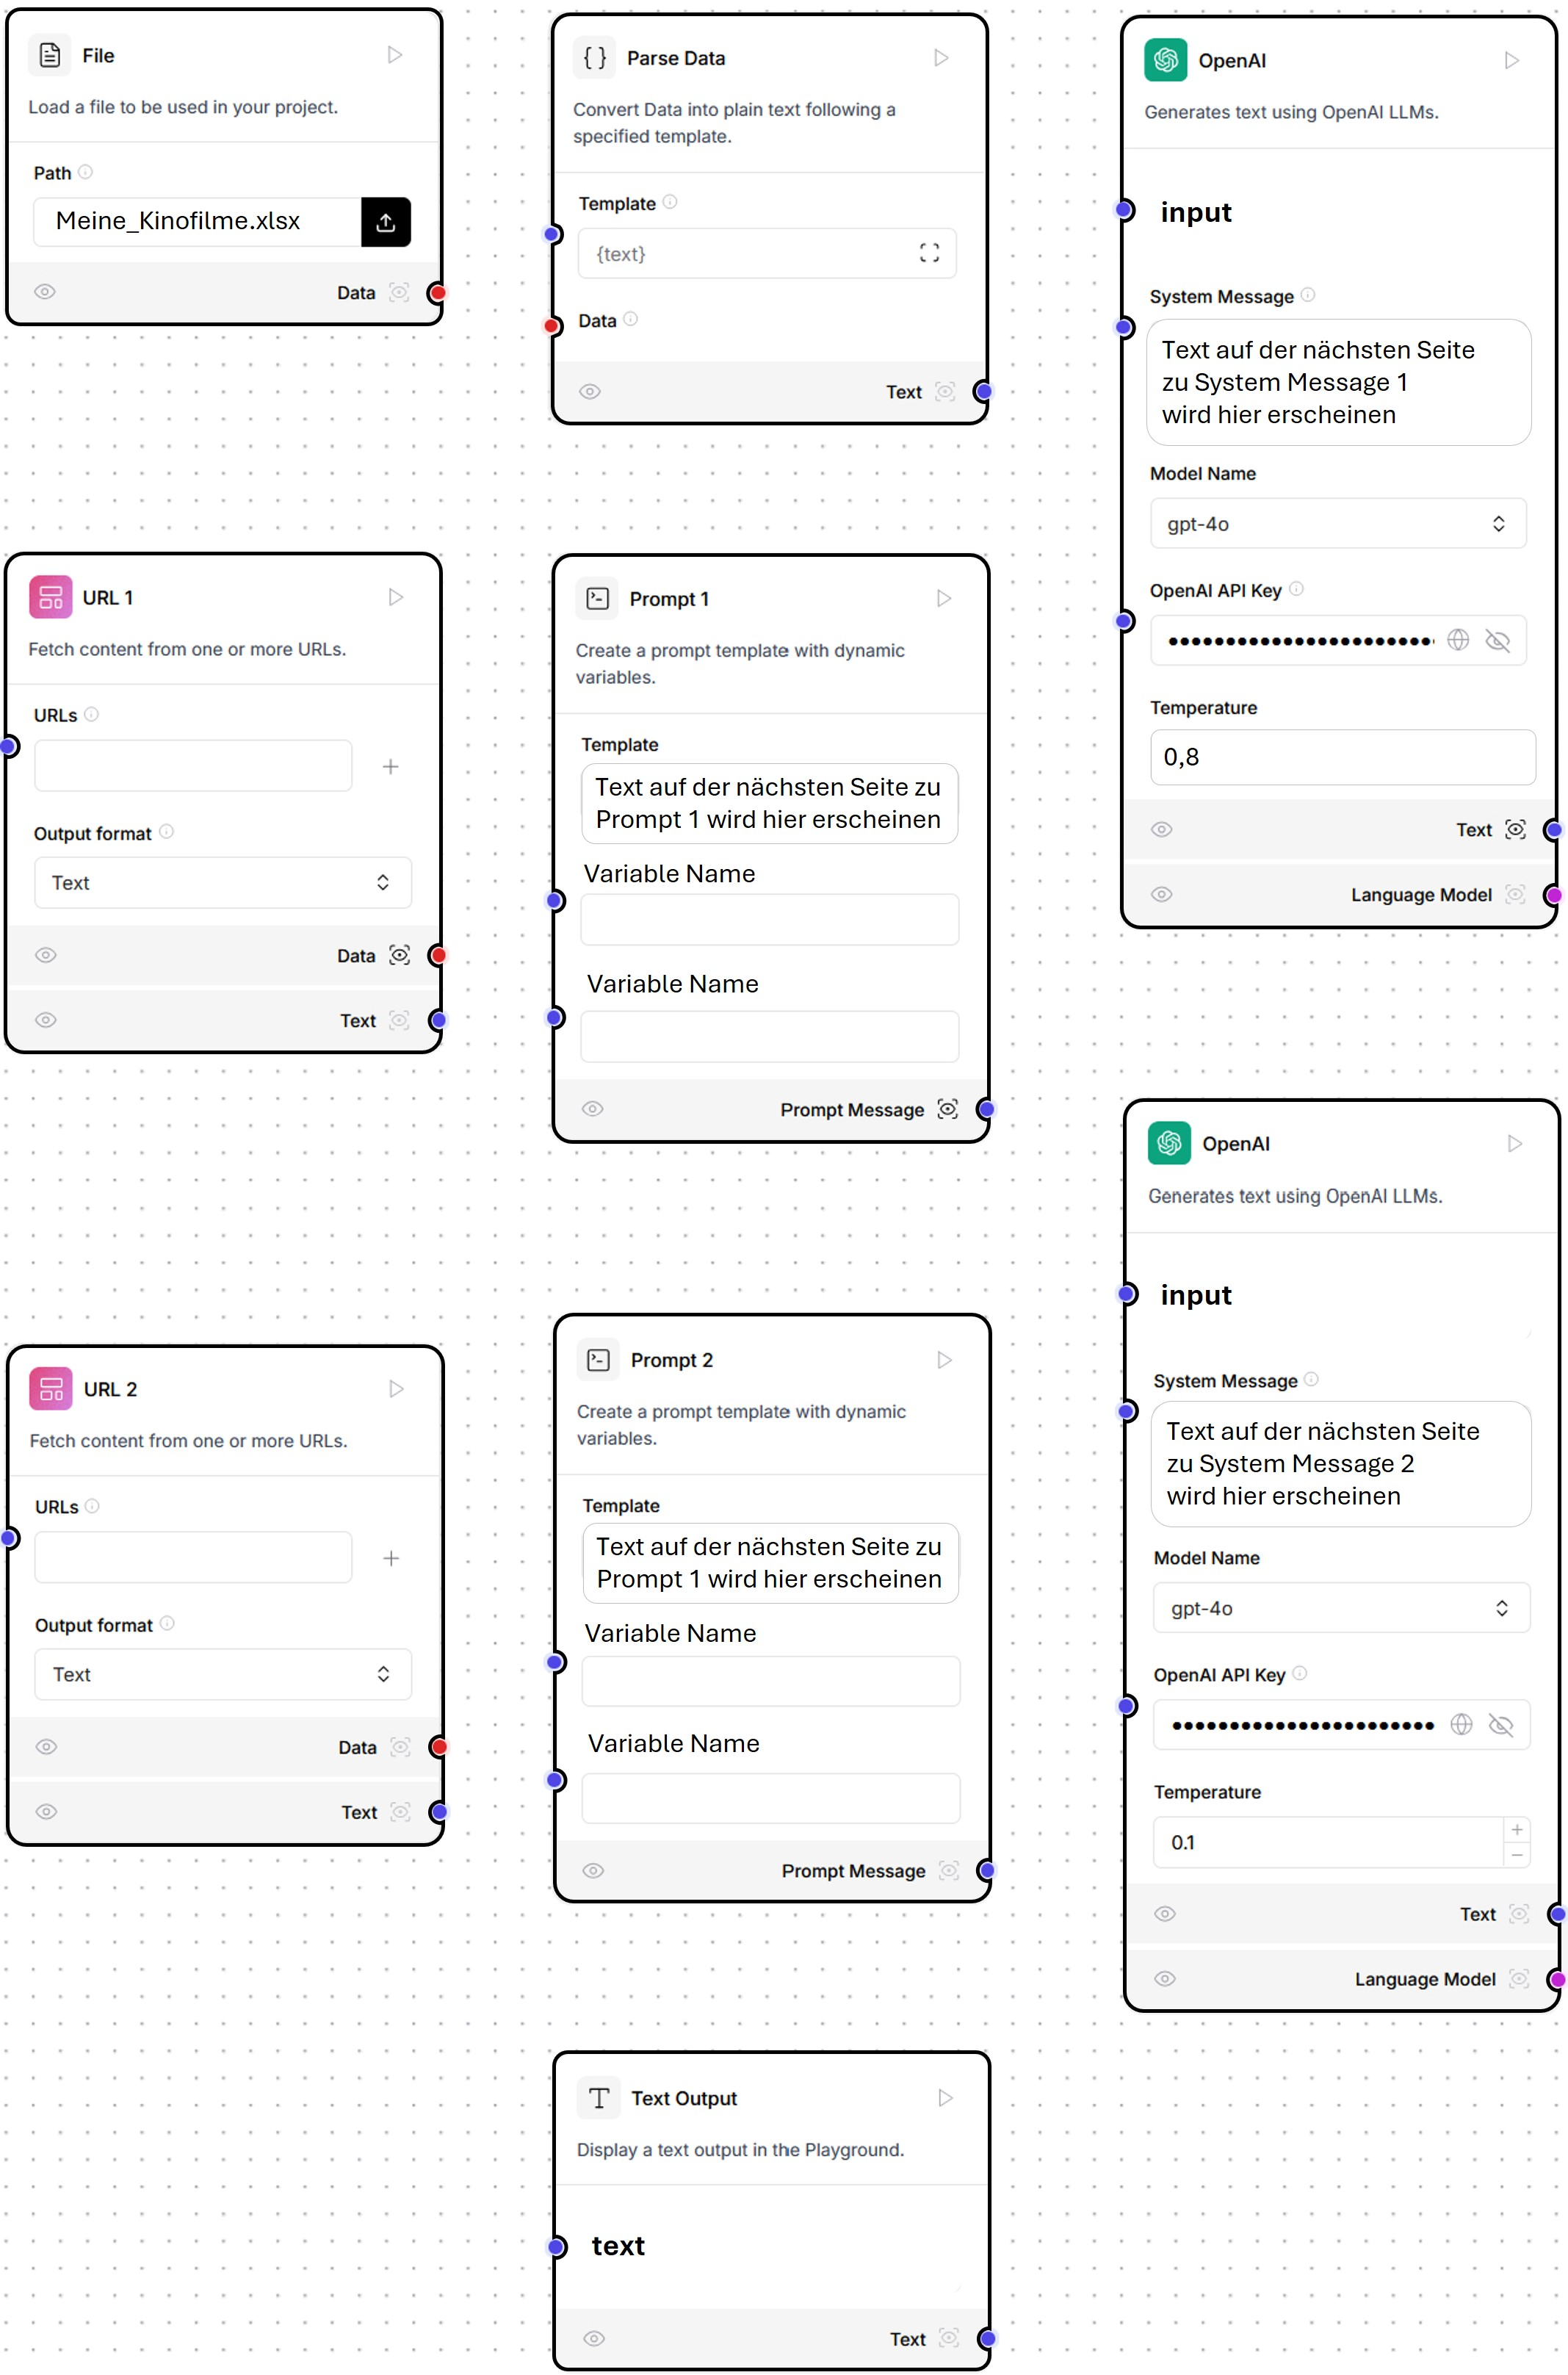
\includegraphics[width=0.95\linewidth]{media_nk/Aufgabe 6/Langflow.jpg}
    %     \caption{Aufgabe 6}
    %     \label{fig:Aufgabe-6}
    % \end{figure}

	\begin{solution}
		\noindent
            \begin{figure}[h!]
                \centering
                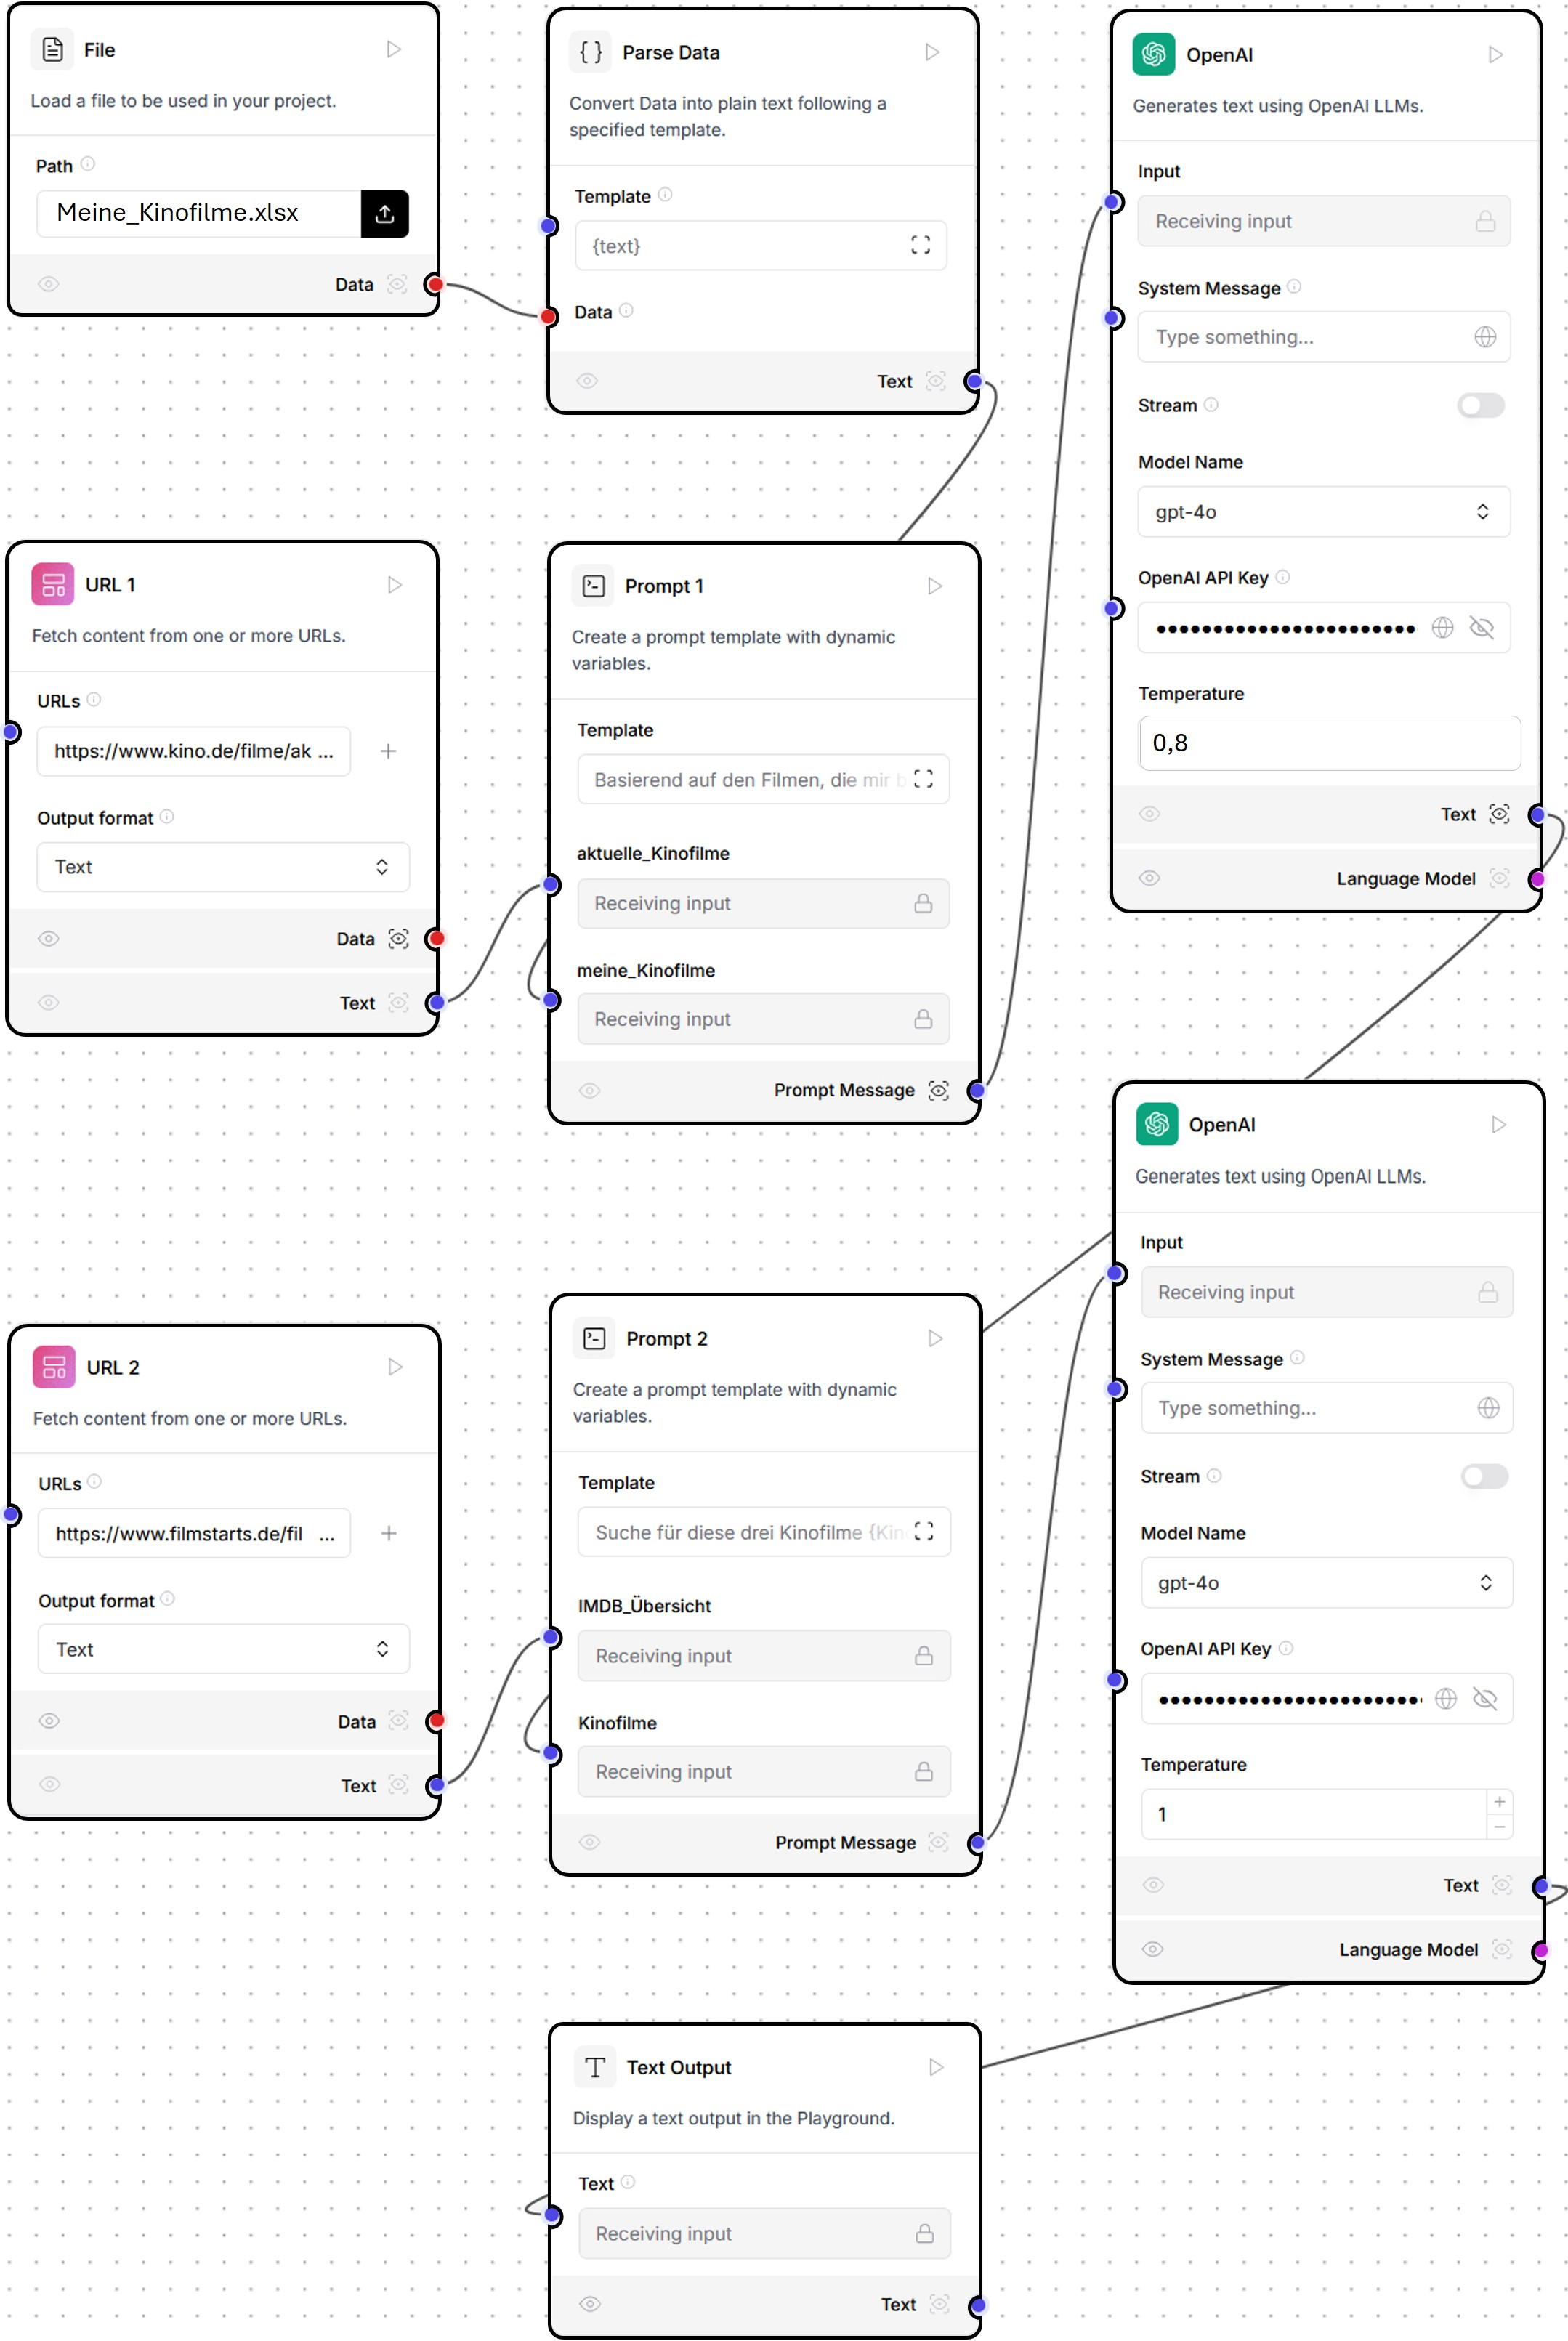
\includegraphics[width=0.95\linewidth]{media_nk/Aufgabe 6/Langflow-Loesung.jpg}
                \caption{Aufgabe 6: Lösung}
                \label{fig:Aufgabe-6-Lösung}
            \end{figure}
	\end{solution}

    \newpage

    % Aufgabenteil b
    \begin{enumerate}[b)]
		\item 
			\begin{minipage}[t]{\linewidth}
				\vspace{-0.61em}
				\begin{wrapfigure}[2]{r}{0.18\linewidth} 
					\raggedleft
					\texttt{(5 Punkt)}
				\end{wrapfigure}
                Erstellen Sie die System Messages und Prompts. Input-Variablen müssen initialisiert und mit geschwungen Klammern verwendet werden, z.B. \{variable\_name\}:
			\end{minipage}
	\end{enumerate}

    \vspace{1cm}

    System Message 1 - dieser Text wird für die \textbf{obere Langflow Komponente OpenAI-Input} verwendet (1 Punkt):\\
    \begin{answerbox}
		\noindent
		\fbox{\parbox[c]{\textwidth}{
				\vspace{3cm}
				\hspace{\textwidth}
		}}\\
	\end{answerbox}
	\begin{solution}
		\noindent
		\fbox{\parbox[c]{\textwidth}{
				\small
				\begin{tabular}{cp{13cm}}
					Beispiele: & Verhalte dich als ein Experte für Filme.\\
                    & Verhalte dich als ein Experte von Empfehlungssystemen.\\
                    1 & Ein Punkt, falls der System Prompt sinnvoll ist. Das ist er, wenn eines dieser drei Kriterien für System Prompts erfüllt ist: Role Injection, Arbeitsanweisungen, Input oder Output Definitionen.
				\end{tabular}
				\hspace{\textwidth}
		}}\\
	\end{solution}
    \vspace{1cm}
    
    Prompt 1 (1,5 Punkte) – Erstellen Sie den ersten Prompt. Dieser Text wird als Text für die Langflow Komponente \textbf{Prompt 1} verwendet. Input-Variablen müssen initialisiert und mit geschwungen Klammern verwendet werden, z.B. \{variable\_name\}:\\
    \begin{answerbox}
		\noindent
		\fbox{\parbox[c]{\textwidth}{
				\vspace{3cm}
				\hspace{\textwidth}
		}}\\
	\end{answerbox}
    \begin{solution}
		\noindent
		\fbox{\parbox[c]{\textwidth}{
				\small
				\begin{tabular}{cp{13cm}}
					Beispiel: & Basierend auf den Filmen, die mir bisher gefallen haben \textit{\{meine\_Kinofilme\}}, empfehle mir 3 aktuelle Filme aus dieser Übersicht: \textit{\{aktuelle\_Kinofilme\}}.\\
                    0,5 & pro sinnvoller Variablenbezeichnung, die ebenfalls in der Langflow Komponente eingetragen wurde (insgesamt 2 Variablen)\\
                    0,5 & für sinnvolles prompten unter Nutzung der Variablen.
				\end{tabular}
				\hspace{\textwidth}
		}}\\
	\end{solution}
    \vspace{1cm}

    System Message 2 - dieser Text wird für die \textbf{untere Langflow Komponente OpenAI-Input} verwendet (1 Punkt):\\
    \begin{answerbox}
		\noindent
		\fbox{\parbox[c]{\textwidth}{
				\vspace{3cm}
				\hspace{\textwidth}
		}}\\
	\end{answerbox}
	\begin{solution}
		\noindent
		\fbox{\parbox[c]{\textwidth}{
				\small
				\begin{tabular}{cp{13cm}}
					Beispiel: & Arbeite strukturiert, lasse dir Zeit und überprüfe deine Ergebnisse auf Richtigkeit.\\
                    & Verhalte dich als ein Experte von Empfehlungssystemen.\\
                    1 & Ein Punkt, falls der System Prompt sinnvoll ist. Das ist er, wenn eines dieser drei Kriterien für System Prompts erfüllt ist: Role Injection, Arbeitsanweisungen, Input oder Output Definitionen.
				\end{tabular}
				\hspace{\textwidth}
		}}\\
	\end{solution}
    \vspace{1cm}

    Prompt 2 (1,5 Punkte) – Erstellen Sie den zweiten Prompt. Dieser Text wird als Text für die Langflow Komponente \textbf{Prompt 2} verwendet. Input-Variablen müssen initialisiert und mit geschwungen Klammern verwendet werden, z.B. \{variable\_name\}:\\
    \begin{answerbox}
		\noindent
		\fbox{\parbox[c]{\textwidth}{
				\vspace{3cm}
				\hspace{\textwidth}
		}}\\
	\end{answerbox}
  	\begin{solution}
		\noindent
		\fbox{\parbox[c]{\textwidth}{
				\small
				\begin{tabular}{cp{13cm}}
					Beispiel: & Suche für diese drei Kinofilme \textit{\{Kinofilme\}} die Bewertung auf dieser Übersicht \textit{\{IMDB\_Übersicht\}} und empfehle mir den Film mit der besten Bewertung.\\
                    0,5 & pro sinnvoller Variablenbezeichnung, die ebenfalls in der Langflow Komponente eingetragen wurde (insgesamt 2 Variablen)\\
                    0,5 & für sinnvolles prompten unter Nutzung der Variablen.
				\end{tabular}
				\hspace{\textwidth}
		}}\\
	\end{solution}

\end{document}
